\documentclass[11pt,a4paper]{article}

% IMPORTS ---------------------------------------

% FONTE E TIPOGRAFIA --------------------

\usepackage{fontspec}

\setmainfont{Poppins}[
  Path = ../../../shared/fonts/poppins/,
  Extension = .ttf,
  UprightFont = Poppins-Regular,
  BoldFont = Poppins-Bold,
  ItalicFont = Poppins-Italic,
  BoldItalicFont = Poppins-BoldItalic
]

\newfontfamily\opensansfont{Open Sans}[
  Path = ../../../shared/fonts/opensans/,
  Extension = .ttf,
  UprightFont = OpenSans-Regular,
  BoldFont = OpenSans-Bold,
  ItalicFont = OpenSans-Italic,
  BoldItalicFont = OpenSans-BoldItalic
]

% IDIOMA E TEXTO GERAL ------------------

\usepackage[brazilian]{babel}
\usepackage{microtype}

% LAYOUT GERAL --------------------------

\usepackage{fancyhdr}
\usepackage{multicol}
\usepackage{parskip}
\usepackage[
a4paper,
top=2cm,
bottom=1.4cm,
left=1.1cm,
right=1.1cm
]{geometry}

% CORES E VISUAL ------------------------

\usepackage{tcolorbox}
\tcbuselibrary{skins,breakable}
\usepackage{tikz}

% IMAGENS E LINKS -----------------------

\usepackage{graphicx}
\usepackage[hidelinks]{hyperref}
\usepackage{refcount}
\usepackage{bookmark}
 
\usepackage{titlesec}
\usepackage{enumitem}

% MATEMATICA ------------------------------

\usepackage{amsmath}
\usepackage{amssymb}

% TABELAS ----------------------------------

\usepackage{booktabs}
\definecolor{HypeOrange}{RGB}{230,122,59}
\definecolor{HypePurple}{RGB}{95,20,120}
\definecolor{HypePurple2}{RGB}{120,12,64}
% Evita que o LaTeX estique o conteúdo verticalmente para preencher a página
\raggedbottom

% Espaço entre colunas, linha separadora e tolerâncias de layout
\setlength{\columnsep}{0.8cm}
\setlength{\emergencystretch}{3em}
\setlength{\columnseprule}{0.4pt}
\setlength{\hfuzz}{2pt}

% Espaço reservado para cabeçalho e rodapé
\setlength{\headheight}{21pt}
\setlength{\footskip}{30pt}

% Cor da linha separadora entre as colunas
\def\columnseprulecolor{\color{gray!40}}

% Ativa o estilo de página customizado e limpa os defaults
\pagestyle{fancy}
\fancyhf{}

% CABEÇALHO ----------------------------------------------------------

\fancyhead[L]{\textcolor{HypePurple}{\textbf{Tá no Hype}}}
\fancyhead[R]{\textcolor{HypePurple}{\textbf{\edicaoMes\ \edicaoAno}}}

% Remove a linha horizontal padrão do fancyhdr
\renewcommand{\headrulewidth}{0pt}

% Barra gradiente centralizada abaixo do cabeçalho
\fancyhead[C]{
\begin{tikzpicture}[remember picture,overlay]
\shade[left color=HypeOrange,right color=HypePurple]
(-0.5\textwidth,-0.18cm) rectangle (0.5\textwidth,-0.09cm);
\end{tikzpicture}
}

% RODAPÉ ------------------------------------------------------------------

% Imagem centralizada no rodapé
\fancyfoot[C]{

\includegraphics[trim=30 18 42 12, clip, height=0.9cm]{../../../shared/assets/rodape.png}
}
\newcounter{hypeartigo}

\newcommand{\hypeartigoanchor}{%
  \refstepcounter{hypeartigo}%
  \edef\hypeartigokey{art:\ifnum\value{hypeartigo}<10 0\fi\arabic{hypeartigo}}%
  \expandafter\label\expandafter{\hypeartigokey}%
  \expandafter\hypertarget\expandafter{\hypeartigokey}{}%
}

% CABEÇALHO DE ARTIGO ------------------------------------

\newcommand{\articleheader}[2]{

\begin{tcolorbox}[
colback=HypeOrange,
colframe=HypeOrange,
arc=0mm,
boxrule=0pt,
left=3mm,
right=3mm,
top=2.5mm,
bottom=2.5mm,
halign=left,
]

{\color{white}
\opensansfont
\raggedright
\fontsize{18}{20}\selectfont
\bfseries
#1\par
}

\end{tcolorbox}
{\small\color{HypePurple} Texto por #2}

\vspace{0.2cm}

}

% MACRO: ARTIGO -----------------------------------------

\newcommand{\hypearticle}[3]{

\hypeartigoanchor

\vspace{0.1cm}

\articleheader{#1}{#2}

#3

\vspace{0.5cm}

}

% MACRO: HYPE EXPLICA (banner manual + corpo de artigo)

\newcommand{\hypeexplica}[3]{

\hypeartigoanchor

\vspace{0.1cm}

\begin{center}
\includegraphics[width=\columnwidth]{#1}
\end{center}
{\small\color{HypePurple} Texto por #2}
\vspace{0.2cm}

#3

\vspace{0.5cm}

}

% MACRO: SUBTÍTULO -------------------------------------

\newcommand{\subtitle}[1]{

\vspace{0.4cm}

{\large\bfseries #1}

}

% MACRO: BLOCO DE DESTAQUE -----------------------------

\newcommand{\highlight}[1]{

\vspace{0.3cm}

\begin{tcolorbox}[
  colback=HypePurple!10,
  colframe=HypePurple!30,
  boxrule=0.4pt,
  arc=3pt,
  left=6pt, right=6pt,
  top=6pt, bottom=6pt,
]
#1
\end{tcolorbox}

}

% MACRO: FONTE ORIGINAL --------------------------------

\newcommand{\originalsource}[1]{

\vspace{0.15cm}


{\color{HypePurple2}Gostou do texto?}\\
Confira também a fonte original principal
\href{#1}{{\color{HypeOrange}aqui}}.

}

% MACRO: OUTRAS FONTES ----------------------------------

% IMAGEM ------------------------------------------------

\newcommand{\articleimage}[3]{

\begin{center}

\includegraphics[width=#1\columnwidth]{#2}

\end{center}
{\small\color{gray}Legenda: #3}

}

% MACRO: BULLET POINTS -----------------------------------

\newenvironment{hypeitemize}
{
\begin{itemize}[
leftmargin=2.5em,
itemsep=0.01em,
topsep=0.1em,
label=\textcolor{HypeOrange}{\Large\textbullet}
]
}
{
\end{itemize}
}

% BOX INFORMATIVO ------------------------------------------

\newtcolorbox{infobox}{
colback=HypeOrange!12,
colframe=HypeOrange!40,
boxrule=0.5pt,
arc=2mm,
left=2mm,
right=2mm,
top=1mm,
bottom=1mm
}

% TESTE DE SUMÁRIO -----------------------------------------

\makeatletter
\newcommand{\summaryitem}[4]{
\bookmark[dest=art:#1,level=0]{#2}%
\hyper@linkstart{link}{art:#1}%
\begin{tcolorbox}[
    colback=white, colframe=white, boxrule=0pt,
    arc=4mm, left=4mm, right=4mm, top=3mm, bottom=3mm
]

\begin{minipage}[c]{0.12\linewidth}
    {\fontsize{28}{28}\selectfont
    \color{HypeOrange}\textbf{#1}}
\end{minipage}
\hfill
\begin{minipage}[c]{0.68\linewidth}
    {\Large\color{HypePurple}\textbf{#2}}

    \vspace{0.15cm}

    #3
\end{minipage}
\hfill
\begin{minipage}[c]{0.12\linewidth}
    \raggedleft
    {\fontsize{28}{28}\selectfont
    \color{HypePurple}\textbf{\ifcsname r@art:#1\endcsname\ifnum\getpagerefnumber{art:#1}<10 0\fi\pageref*{art:#1}\else #4\fi}}

    {\small\color{HypeOrange}\textbf{pág.}}
\end{minipage}

\end{tcolorbox}%
\hyper@linkend

\vspace{0.3cm}
}
\makeatother

% MACRO: FEEDBACK DA EDIÇÃO ------------------------------

\newcommand{\hypefeedback}[1]{
\begin{center}
\href{#1}{
\includegraphics[width=1.0\columnwidth]{../../../shared/assets/final.png}}
\end{center}
}

% DOCUMENTO -------------------------------------

\begin{document}

\sloppy

\newcommand{\edicaoMes}{OUTUBRO}
\newcommand{\edicaoAno}{2026}

% CAPA BONITA -----------------

% PÁGINA 1: CAPA (imagem em tela cheia) ---------------------------
\thispagestyle{empty}
\null
\begin{tikzpicture}[remember picture,overlay]
  \node[inner sep=0pt,anchor=south west] at (current page.south west)
    {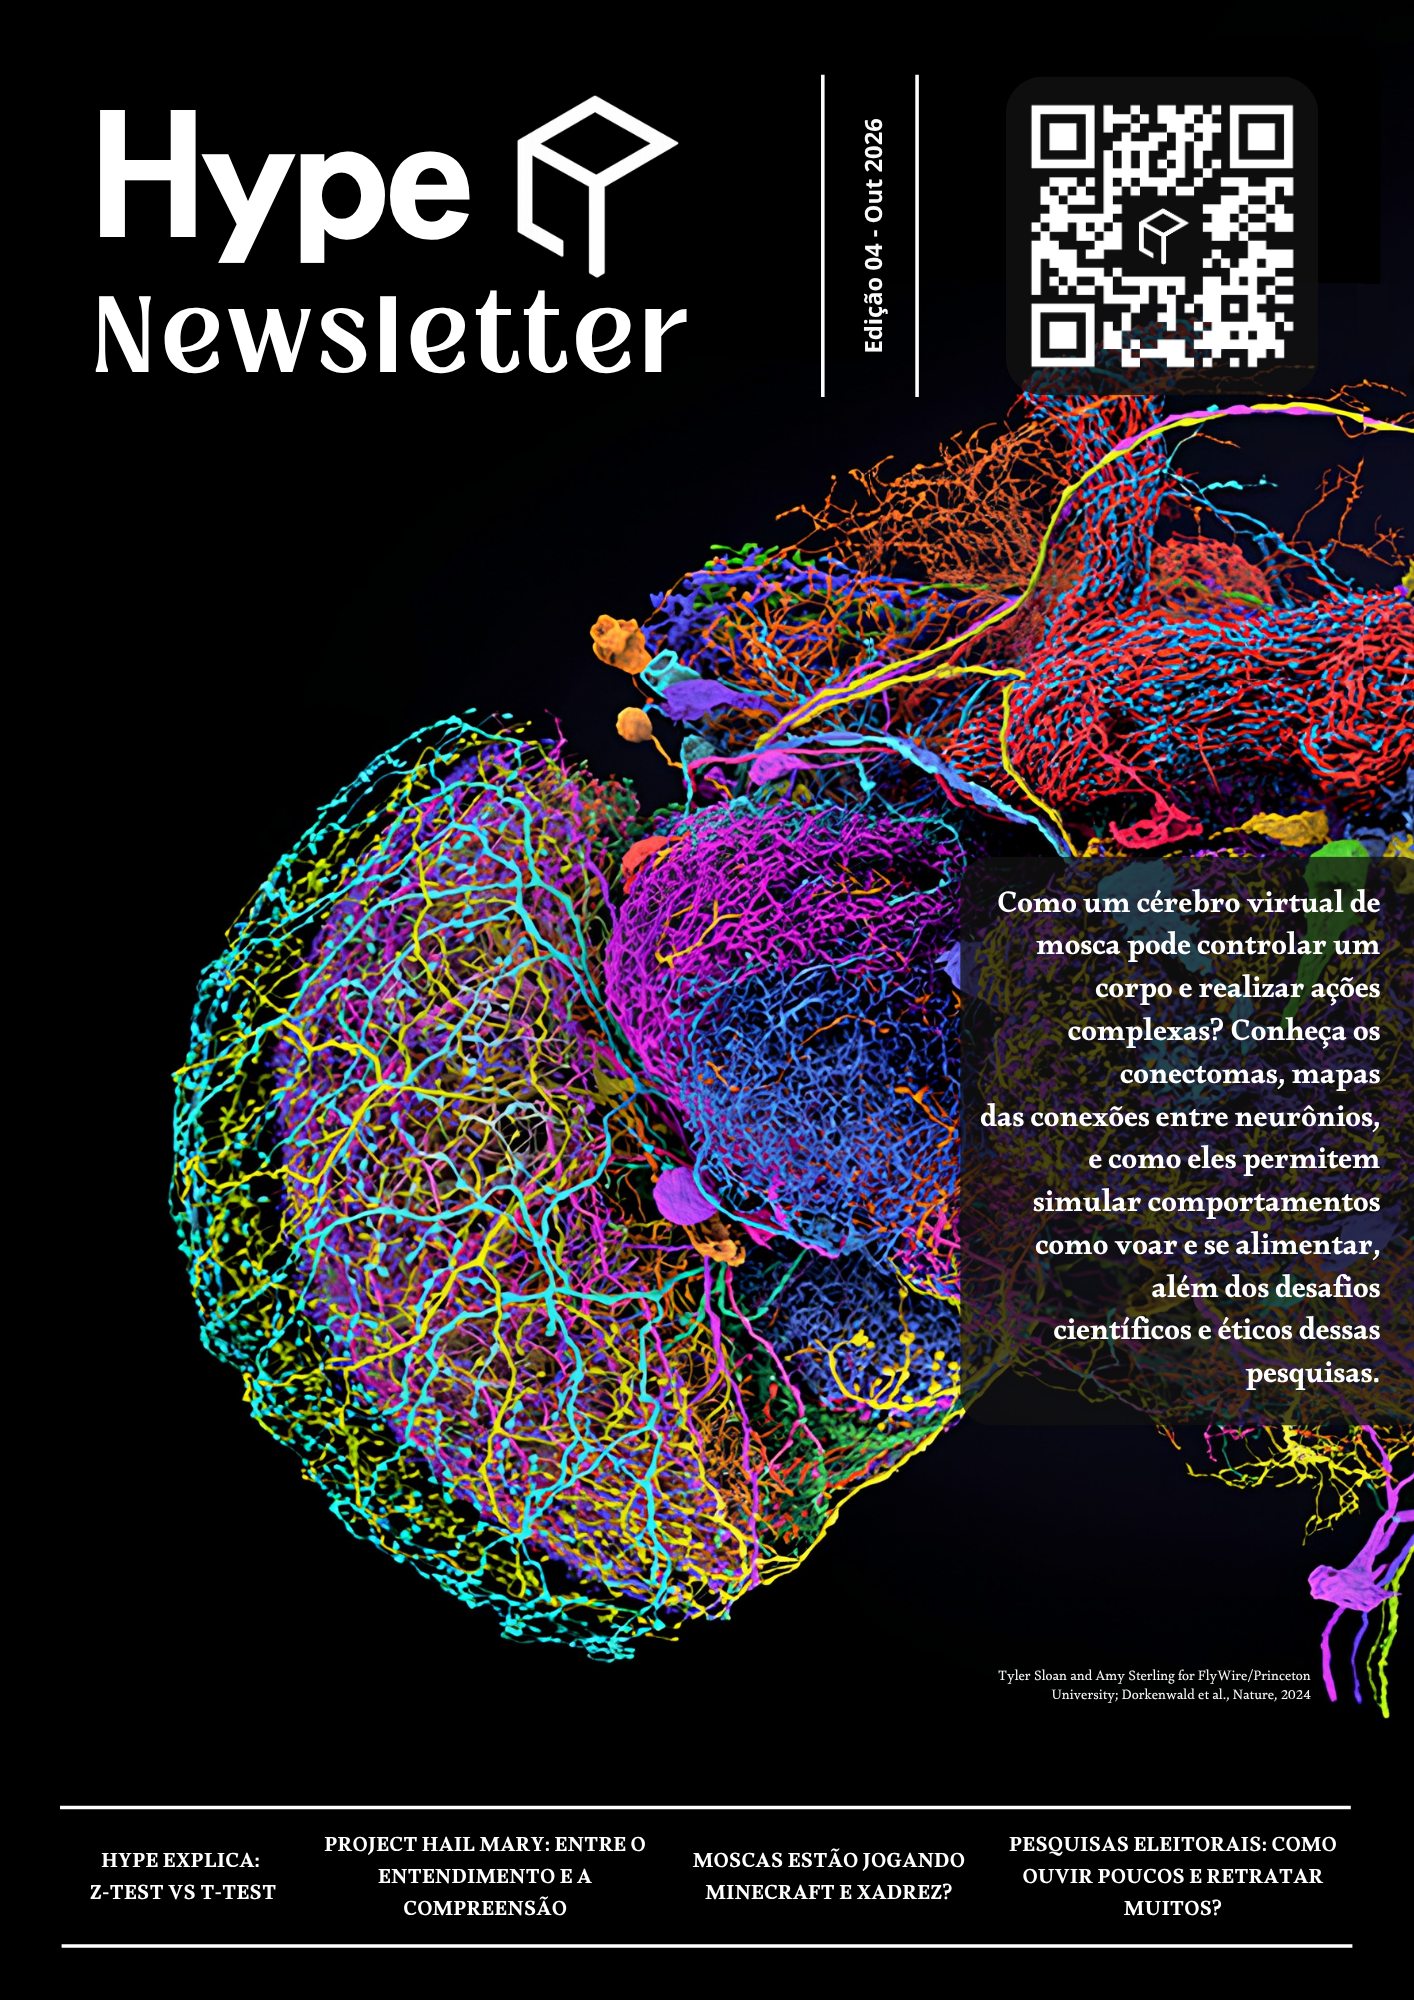
\includegraphics[width=\paperwidth,height=\paperheight]{../styles/capa.png}};
\end{tikzpicture}
\clearpage

% PÁGINA 2: SUMÁRIO ------------------------------------------------

\begin{minipage}[t]{0.48\textwidth}


\includegraphics[width=0.65\textwidth]{../../../shared/assets/logo.png}

\end{minipage}
\hfill
\begin{minipage}[t]{0.48\textwidth}

\vspace{-2.0cm}

\raggedleft

{\fontsize{26}{28}\selectfont
\bfseries
\color{HypeOrange}
\edicaoMes
}

\vspace{0.1cm}

{\fontsize{22}{24}\selectfont
\bfseries
\color{HypePurple}
\edicaoAno
}

\end{minipage}

\vspace{0.3cm}

%\begin{center}

% \includegraphics[width=0.5\textwidth]{../shared/assets/capa.png}

% \end{center}


\vspace{1.5cm}

\summaryitem
{01}
{Hype Explica: z-test vs t-test}
{O \textit{z-test} e o \textit{t-test} podem parecer quase iguais, mas existe uma diferença importante entre eles! Principalmente o quanto sabemos sobre a população. Entenda quando cada um é usado e por que essa escolha pode mudar os resultados.}
{03}

\summaryitem
{02}
{Project Hail Mary: Entre o entendimento e a compreensão}
{Muito além de traduzir palavras isoladas, uma boa tradução precisa considerar as relações entre elas. É essa capacidade que torna os \textit{Transformers} tão importantes para a inteligência artificial e que nos faz imaginar como a comunicação entre Grace e Rocky (em \textit{Devoradores de Estrelas}) poderia ser diferente.}
{05}

\summaryitem
{03}
{Moscas estão jogando Minecraft e Xadrez?}
{Como um cérebro virtual de mosca pode controlar um corpo e realizar ações complexas? Conheça os conectomas, mapas das conexões entre neurônios, e como eles permitem simular comportamentos como voar e se alimentar, além dos desafios científicos e éticos dessas pesquisas.}
{06}

\summaryitem
{04}
{Pesquisas eleitorais: Como ouvir poucos e retratar muitos?}
{Como uma pesquisa com poucos milhares pessoas pode representar milhões de eleitores? Entenda como a seleção da amostra e a margem de erro ajudam a estimar a intenção de voto.}
{08}

\pagebreak

\vspace{0.3cm}

% CONTEÚDO ---------------------

%\raggedcolumns
\begin{multicols}{2}
%\raggedcolumns

\hypeexplica{../sections/hype-explica-z-vs-t/banner-hype-explica.png}
{Gustavo Neves Moraes}
{

\hspace*{1.5em}
Nos cursos introdutórios de estatística, o chamado \textit{z-test} e o \textit{t-test}, que costumam aparecer lado a lado,
com fórmulas praticamente idênticas e valores críticos distintos.
No entanto, a diferença entre eles não é apenas operacional,
pois está relacionada ao que se conhece sobre a população antes de a análise começar
e à incerteza que acompanha essa informação.

\subtitle{O teste de hipótese para a média}

\hspace*{1.5em}
Um teste de hipótese para a média responde a uma simples pergunta:
\highlight{A média observada na amostra, $\bar{x}$, é compatível com o valor de referência $\mu_0$, afirmado pela hipótese nula?}
Como duas amostras da mesma população raramente têm a mesma média,
alguma diferença entre $\bar{x}$ e $\mu_0$ é esperada mesmo quando $H_0$ é verdadeira.
O que o teste avalia é se essa diferença é pequena o bastante para ser atribuída ao acaso
ou grande demais para isso.

\hspace*{1.5em}
Para medir o tamanho da diferença, ela é expressa em unidades de erro padrão,
que indicam o quanto uma média amostral costuma variar de uma amostra para outra.
O resultado é a estatística de teste,
um número que informa a quantos erros padrão a média observada está de $\mu_0$.
Essa estatística é então comparada com um valor crítico, definido pelo nível de significância $\alpha$,
e, se ela o ultrapassa, rejeita-se $H_0$.

\hspace*{1.5em}
O valor crítico, por sua vez, depende da distribuição que a estatística segue quando $H_0$ é verdadeira.
É exatamente nesse ponto que o \textit{z-test} e o \textit{t-test} se separam.

\subtitle{Dois testes, uma diferença}

\hspace*{1.5em}
O erro padrão da média depende do desvio padrão populacional $\sigma$.
No \textit{z-test}, esse parâmetro é considerado conhecido,
e a estatística de teste segue a distribuição normal padrão:

\[
z = \frac{\bar{x} - \mu_0}{\sigma / \sqrt{n}}
\]

\hspace*{1.5em}
No \textit{t-test}, $\sigma$ é desconhecido e substituído pelo desvio padrão amostral $s$.
A fórmula tem a mesma aparência, mas a estatística passa a seguir a distribuição t de Student,
com $n - 1$ graus de liberdade:

\[
t = \frac{\bar{x} - \mu_0}{s / \sqrt{n}}
\]

\begin{hypeitemize}
    \item \textbf{\textit{z-test}:} $\sigma$ conhecido, distribuição normal padrão.
    \item \textbf{\textit{t-test}:} $\sigma$ estimado por $s$, distribuição t de Student.
\end{hypeitemize}

\subtitle{Por que as caudas são mais pesadas?}

\hspace*{1.5em}
No \textit{z-test}, o único elemento que varia de uma amostra para outra é a média $\bar{x}$,
pois o desvio padrão $\sigma$ é um valor fixo e conhecido.
No \textit{t-test}, o desvio padrão amostral $s$ também é calculado a partir dos dados
e, portanto, muda a cada amostra.
Isso significa que o denominador da estatística passa a ser uma fonte extra de variação.

\hspace*{1.5em}
Essa variação adicional importa porque $s$ às vezes subestima $\sigma$ por puro acaso.
Quando isso acontece, o erro padrão calculado fica menor do que deveria,
e a estatística resultante se afasta de zero mais do que o esperado,
mesmo com $H_0$ verdadeira.
Em amostras pequenas, $s$ oscila bastante,
então esses valores extremos aparecem com mais frequência do que a distribuição normal prevê.

\hspace*{1.5em}
A distribuição t de Student incorpora esse efeito por meio de caudas mais pesadas,
ou seja, atribui mais probabilidade aos valores extremos.
Como consequência, os valores críticos são maiores,
e o critério para rejeitar $H_0$ se torna mais exigente,
o que compensa a incerteza de ter estimado $\sigma$ a partir de poucos dados.

% \articleimage{1.0}{../sections/hype-explica-z-vs-t/distribution.png}{AA}

\subtitle{Graus de liberdade e convergência}

\hspace*{1.5em}
O formato da distribuição t é determinado pelos graus de liberdade,
que no teste para uma única média valem $n - 1$.
Com poucos graus de liberdade, as caudas se afastam bastante das da normal,
e, à medida que $n$ aumenta, $s$ passa a estimar $\sigma$ com mais precisão,
de modo que a distribuição t converge para a normal padrão.
A figura e a tabela a seguir ilustram esse comportamento.

\articleimage{1.0}{../sections/hype-explica-z-vs-t/curvas-z-t.png}{Distribuição normal padrão comparada a distribuições t com 2, 5 e 30 graus de liberdade.}

\resizebox{\linewidth}{!}{%
\begin{tabular}{|cccc|}
\hline
\textbf{\small Amostra ($n$)} & \textbf{Graus de liberdade} & \textbf{Valor crítico t} & \textbf{Valor crítico z} \\
\hline
5   & 4   & 2,776 & 1,960 \\
10  & 9   & 2,262 & 1,960 \\
30  & 29  & 2,045 & 1,960 \\
100 & 99  & 1,984 & 1,960 \\
\hline
\end{tabular}%
}

\vspace{0.4em}
{\small Valores críticos bilaterais para $\alpha = 0{,}05$.}

\hspace*{1.5em}
Para $n = 5$, o valor crítico t é cerca de 40\% maior que o z,
enquanto para $n = 100$ a diferença é inferior a 2\%.
A distância entre os dois testes, portanto, é relevante principalmente em amostras pequenas.

\subtitle{Um exemplo numérico}

\hspace*{1.5em}
Considere uma amostra de $n = 5$ observações, com média $\bar{x} = 108$ e desvio padrão $s = 8$,
usada para testar $H_0: \mu = 100$ com $\alpha = 0{,}05$.
O erro padrão é $8/\sqrt{5} \approx 3{,}58$,
e a estatística de teste vale $(108 - 100)/3{,}58 \approx 2{,}24$.

\hspace*{1.5em}
Se $s$ for tratado como se fosse $\sigma$ e comparado ao valor crítico z de 1,96,
a conclusão é rejeitar $H_0$, com p-valor em torno de 0,025.
Ao utilizar o valor crítico t para 4 graus de liberdade, que é 2,776,
não há evidência suficiente para rejeitar $H_0$, e o p-valor passa a ser aproximadamente 0,09.
Os mesmos dados conduzem a conclusões opostas,
e apenas a segunda leva em conta que o desvio padrão foi estimado a partir de cinco observações.

\vspace{12mm}
\subtitle{Quando cada teste se aplica}

\hspace*{1.5em}
O \textit{z-test} é adequado quando $\sigma$ é de fato conhecido,
situação rara, que costuma ocorrer em processos industriais com longo histórico de calibração.
Ele também é o procedimento padrão para proporções,
caso em que a variância é determinada pela própria proporção testada
e não precisa ser estimada separadamente.
Para médias com $\sigma$ desconhecido, que é o cenário usual em ciência de dados,
o \textit{t-test} é o procedimento apropriado.

\subtitle{Uma ressalva importante}

\hspace*{1.5em}
A regra segundo a qual $n \geq 30$ autoriza o uso do \textit{z-test} é uma convenção histórica,
associada à época em que as tabelas eram impressas e consultadas manualmente.
Com $n$ grande, a diferença entre os dois testes se torna desprezível,
e, como os softwares estatísticos calculam o \textit{t-test} sem custo adicional,
a prática atual é utilizá-lo sempre que $\sigma$ for desconhecido.
Vale lembrar ainda que, em amostras pequenas, o \textit{t-test} pressupõe uma população aproximadamente normal,
condição que deve ser verificada antes de se confiar no resultado.

\begin{infobox}
\textbf{Curiosidade:}\\
A distribuição t foi proposta por William Sealy Gosset em 1908,
quando trabalhava na cervejaria Guinness, em Dublin,
e a empresa o obrigou a publicar sob o pseudônimo \textit{Student}.
Ele precisava tirar conclusões a partir de lotes pequenos de cevada e de cerveja,
um contexto em que as aproximações normais não funcionavam bem.\\
\textbf{\href{https://www.instagram.com/p/Dexi6WNFQJu/}{link do vídeo sobre a curiosidade aqui.}}
\end{infobox}

\vspace{0.1em}
{\color{HypePurple2} Quer se aprofundar mais?}

\href{https://www.open.edu/openlearn/science-maths-technology/data-analysis-hypothesis-testing/content-section-6.1}{- Data analysis: hypothesis testing} \\
\href{https://www.jstor.org/stable/2331554?origin=crossref}{- Student (1908), The Probable Error of a Mean, Biometrika, vol. 6.}

}
\vspace{50mm}
% !TEX root = ../../main/main.tex
\hypearticle
{Project Hail Mary: Entre o entendimento e a compreensão}
{Nathália Pereira}
{

\subtitle{O início de tudo}
    \hspace{1cm}No filme \textbf{Project Hail Mary (2026), em português Devoradores de Estrelas}, é descrito
    uma realidade de ficção científica, em que toda forma de vida no planeta Terra encontra-se em risco de extinção devido a uma forma extraterrestre parasita
    que consome o Sol. 

    \hspace{1cm}Um jovem biólogo e professor de ciências, Ryland Grace, foi selecionado para estudar a forma devoradora
    e posteriormente ser lançado em uma missão espacial para estudar e analisar o funcionamento de uma estrela que não foi consumida (Tau Ceti). 
    Nessa jornada, Grace encontra outro ser extraterrestre, declarado por "Rocky", entretanto houve uma barreira a ambos: \textbf{a comunicação.}

    \hspace{1cm}Dessa forma, a base delimitada provocou \textbf{grandes lacunas} para o diálogo fluido e exato entre os seres, e deixou a interpretação de Rocky simples. 

    \hspace{1cm}Dito isso, surge uma grande dúvida:
\subtitle{\begin{infobox} Há como otimizar a tradução?  \end{infobox}}
\subtitle{Os Transformers}
    \hspace{1cm} Por meados de 2017, houve a apresentação do modelo de \textbf{Transformers}, uma ramificação do Deep Learning, pelo artigo científico
    \textbf{"Attention is All you Need"}. O modelo tem revolucionado o processo de tradução a partir de \textbf{mecanismos de atenção}, e consequentemente
    lida com uma linguística complexa por meio de implementação de \textbf{contexto} à sua estrutura.

    \hspace{1cm}De início, é importante apresentar que cada palavra utilizada passa a ser expressada como um \textbf{vetor}, uma vez que por uma modelagem matemática formalizada em
    conjunto do sentido do vetor, o computador aprende a similaridade entre palavras e, posteriormente, sequências. Uma maneira de visualizar
    essa transformação vetorial é pela própria noção de linguagem, já que permite a compreensão entre o humano e o computador.

\subtitle{Mas como funcionam?}
    \hspace{1cm}O padrão é uma arquitetura por \textbf{codificador e decodificador}. 

    \articleimage
    {1.0}
    {/home/nath/newsletter102026/ta-no-hype-newsletter/editions/2026-10/sections/rocky-comunicacao-transformers/foto2.png}
    {Estrutura do modelo de Transformers}

    \hspace{1cm}No codificador, cada palavra da sequencia possui um valor de correlação, ou seja, 
    a partir de cálculos internos, uma recorrência é atribuída para cada posição dentro da frase. Assim o decodificador, pela análise de posições anteriores que a ser trabalhada
    no momento, produz a entrada em conjunto da saída do programa e a computa sequencialmente. 

    \hspace{1cm}Esse mecanismo origina-se das estratégias denominadas \textbf{"Scaled Dot-Product Attention" e "Multi-Head Attention"}, que, respectivamente, se caracteriza por otimizar o cálculo
    da atenção e torná-lo mais eficiente, a partir da formalização de pesos por produtos escalares, enquanto a segunda consiste em trabalhar com diferentes mecanismos de atenção em paralelo,
    combinando seus resultados posteriormente. 

    \hspace{1cm}Por consequência, é permitido ao modelo analisar diferentes representações de uma mesma palavra em função de sua posição e do contexto da frase, identificando relações entre 
    as palavras e atribuindo-lhes diferentes níveis de importância. 
    
    \hspace{1cm}Dessa forma, o contexto é construído e utilizado continuamente pelo modelo, que prevê a próxima palavra com base nas palavras anteriores.

    \articleimage
    {1.0}
    {/home/nath/newsletter102026/ta-no-hype-newsletter/editions/2026-10/sections/rocky-comunicacao-transformers/foto1.png}
    {Scaled Dot-Product Attention e Multi-Head Attention}

\subtitle{Resultados}
    \hspace{1cm} Na tradução de inglês para alemão da World Memory Teste (WMT) em 2014, o qual mede o nível de desempenho intelectual geral e o QI de forma rápida pela memorização, o modelo Transformer
    supera os melhores modelos anteriores de camadas por convolução (CNN) e por recorrencia (RNN) e em mais de 2,0 pontos na métrica Bilingual Evaluation Understudy (BLEU), que é um algoritmo automático usado para avaliar
    a qualidade de textos gerados por computador, de maneira a estabelecer um novo recorde com uma pontuação BLEU de 28,4, sendo essa \textbf{nota considerada altíssima e revolucionária}.

\subtitle{Considerações finais}
    \hspace{1cm}Por fim, penso em como a comunicação entre Grace e Rocky poderia ter sido mais fácil e dinâmica, assim como a troca cultural entre espécies, caso o modelo descrito anteriormente fosse utilizado para elevar
    \textbf{o nível de complexidade e profundidade das relações nesse contexto}. 
    
    \hspace{1cm}Afinal, como disse Nelson Mandela:
    \begin{infobox} "Se você falar com um homem numa linguagem que ele compreende, isso entra na cabeça dele. Se você falar com ele em sua própria
    linguagem, você atinge seu coração."\end{infobox} 
    
    \hspace{1cm}Acredito que essa ideia se aplica a todas as possíveis formas de vida inteligentes existentes.


\originalsource{https://proceedings.neurips.cc/paper_files/paper/2017/file/3f5ee243547dee91fbd053c1c4a845aa-Paper.pdf}

}
% !TEX root = ../../main/main.tex
% Requer \usepackage{wrapfig} no preâmbulo (para a imagem do conectoma ao lado do texto)

\hypearticle
{Moscas estão jogando Minecraft e Xadrez?}
{Matheus Pires}
{

Diversos conteúdos repercutiram ultimamente na internet retratando simulações de moscas realizando múltiplas atividades, desde buscar uma fonte de água para hidratação, até jogar DOOM e poker. Essas simulações realizadas por entusiastas de IA e tecnologia baseiam-se em um estudo científico realizado pelo centro de pesquisa \textit{HHMI Janelia Research Campus}, em parceria com o Google Research, com o objetivo de mapear as conexões neurais e funcionais do cérebro de uma mosca-da-fruta (\textit{Drosophila melanogaster}).

Esse mapeamento cerebral pode ser representado por um \textbf{\textit{conectoma}}, que consiste em grafos direcionados que representam as conexões entre cada neurônio. Para desenvolver esse conectoma, os cientistas tingiram as células do sistema nervoso de uma mosca com metais pesados, extraíram fatias finas e analisaram-nas utilizando um microscópio de alta resolução. As projeções dos neurônios, a partir das imagens capturadas, foram segmentadas e conectadas utilizando visão computacional, cujos resultados foram analisados manualmente ao decorrer de 33 anos, até produzirem a primeira versão oficial do conectoma, entitulada de MaleCNS.

Os estudos englobando os mapeamentos neurais demonstram resultados promissores na interpretação e reação a estímulos em escala praticamente idêntica à de um cérebro real. Exemplificadamente, quando uma mosca está voando, há uma série de neurônios que são ativados e mantêm suas percepções axial e de rotação, e o mesmo padrão de ativação neural é visualizado nos conectomas quando submetidos aos mesmos estímulos.

As sinapses --- relações de conexão entre os neurônios e outras células --- podem ser representadas como uma matriz esparsa, isto é, uma matriz majoritariamente constituída por elementos nulos, ou zeros. Essa relação binária, ativa (1) e inativa (0), dos valores da matriz é o que possibilita representar os estímulos desses neurônios entre excitatórios, regiões sendo ativadas, e inibitórios, regiões sendo inibidas ou desativadas.

\articleimage{0.8}{../sections//mapeamento_cerebral_moscas/assets/conectoma_mosca.png}{Representação virtual do conectoma de uma mosca}


Entretanto, o ponto-chave que permite que as moscas possam jogar xadrez, tocar piano e até mesmo rolar continuamente o feed do Instagram para obter dopamina é a implementação do cordão nervoso central na arquitetura do conectoma. Essa estrutura do organismo é responsável por assegurar as capacidades motoras e sensoriais, assim como a percepção de informações do ambiente externo. O cordão nervoso central é o responsável por permitir as simulações, pois a partir dele é possível estabelecer uma conexão entre um ``cérebro virtual'' e um ``corpo'' para ser controlado.


A matriz que comentamos representa adequadamente as conexões entre os neurônios, no entanto, ela está ausente e carece de algumas informações cruciais que determinam funções e, consequentemente, ações. Essas informações necessárias são, principalmente: a corrente entre as sinapses (tendo em vista que informações nos neurônios são transmitidas através de estímulos elétricos), a intensidade da sinapse e seu tempo de duração, além de outras informações auxiliares.

Com esses dados, se cada neurônio do mapeamento projetado receber em seus parâmetros exatamente os mesmos valores que uma mosca real receberia, então a simulação será capaz de emular os mesmos resultados. Na representação visual exemplificada abaixo, os neurônios sensíveis a açúcar da simulação foram ativados, desencadeando uma cadeia de ativações sinápticas até, em última instância, o ``neurônio motor 9'', responsável pela movimentação da probóscide da mosca, ser ativado. Assim, a mosca da simulação foi capaz de beber uma deliciosa água açucarada (\textit{Yummy}).

\articleimage{1.0}{../sections/mapeamento_cerebral_moscas/assets/neuron_activation_schema.png}{Circuito de iniciação da alimentação: do estímulo de açúcar unilateral ao neurônio motor 9}

Além do âmbito científico, inúmeras discussões acerca dos princípios éticos dessas simulações emergiram conforme novas vertentes foram produzidas: as moscas dessas simulações possuem consciência de algum modo? Elas estão experienciando sofrimento ou dor?

A resposta para tais indagações varia de acordo com a óptica utilizada, entretanto, na definição humana de consciência, as moscas não possuem nenhum nível de senciência e não são capazes de ``sofrer'' ou interpretar uma determinada ação como danosa, ou benéfica, para si própria. Logo, podem permanecer tranquilos, as moscas não irão se revoltar contra a humanidade em um futuro distópico similar ao de ``\textit{I Have No Mouth, and I Must Scream}'' devido às simulações e estudos realizados com a virtualização do cérebro de uma delas.

Pelo contrário, as pesquisas em desenvolvimento contribuirão amplamente para a compreensão de aspectos que desconhecemos acerca de percepção sensorial, aprendizado, memória, síndromes e distúrbios neurológicos que afetam diretamente o sistema nervoso e, consequentemente, a estrutura corporal --- como as doenças de Parkinson e de Alzheimer --- e como medidas de cura e tratamento podem ser implementadas. Com a progressão desses estudos, a humanidade poderá evoluir significativamente nas áreas de saúde, comportamento social, robótica e aprendizado de máquina.
\originalsource{https://www.neuroai.science/p/are-flies-playing-beat-saber}

}

\vspace{20mm}
\hypearticle{Pesquisas eleitorais: Como ouvir poucos e retratar muitos?}
{Gustavo Neves Moraes}
{

\hspace*{1.5em}
Em períodos eleitorais, é comum ver pesquisas que entrevistam cerca de 2 mil pessoas
para descrever a intenção de voto de mais de 150 milhões de eleitores.
A desconfiança acerca dessa desproporção é natural,
mas ela se apoia em uma intuição equivocada de como é feita a seleção.
A precisão de uma pesquisa depende muito mais de como a amostra é escolhida
do que da fração do eleitorado que foi ouvida.

\subtitle{Por que uma amostra pequena pode bastar}

\hspace*{1.5em}
Para entender de forma simplificada, vamos usar uma alusão bastante famosa: 
para saber se uma sopa está no ponto, basta provar uma colherada, desde que a panela esteja bem misturada.
O tamanho da panela não muda isso,
pois o que importa é que a colherada represente o conjunto.

\hspace*{1.5em}
Em uma pesquisa eleitoral, a mistura da sopa corresponde à seleção aleatória, isto é,
quando todo eleitor tem uma chance conhecida de ser escolhido,
a amostra tende a reproduzir as proporções do eleitorado.
Ainda assim, ela não será idêntica à população,
já que cada sorteio produz um grupo ligeiramente diferente do outro.
Essa diferença é meramente fruto do acaso e, por seguir regras matemáticas conhecidas,
pode ser medida e informada junto com o resultado, na forma da margem de erro.

\subtitle{Quanto a amostra pode errar}

\hspace*{1.5em}
Seja $p$ a proporção de eleitores que apoiam determinado candidato.
A proporção observada na amostra, $\hat{p}$, varia de uma amostra para outra,
e essa variação é medida pelo erro padrão.
Para um nível de confiança de 95\%, a margem de erro é aproximadamente:

\[
\text{margem} \approx 1{,}96 \sqrt{\frac{p(1-p)}{n}}
\]

\hspace*{1.5em}
O valor 1,96 vem da distribuição normal padrão.
Para amostras grandes, $\hat{p}$ se distribui aproximadamente como uma normal em torno de $p$,
e, nessa distribuição, cerca de 95\% da probabilidade fica a até 1,96 erros padrão da média.
A margem de erro, portanto, é esse número de erros padrão
multiplicado pelo erro padrão de $\hat{p}$, que é a raiz da fórmula.
Para outros níveis de confiança, o valor muda de acordo com a Tabela da Distribuição Normal (por
exemplo, valores famosos são 1,645 para 90\% e 2,576 para 99\%).

\hspace*{1.5em}
O tamanho da população não aparece na fórmula,
pois, para populações grandes, a precisão é determinada por $n$.
O produto $p(1-p)$ é máximo quando $p = 0{,}5$, e é esse caso que costuma servir de referência.
Como $n$ está dentro da raiz, reduzir a margem pela metade exige quadruplicar a amostra,
o que explica por que a maioria das pesquisas se limita a alguns milhares de entrevistados.

\subtitle{Um exemplo numérico}

\hspace*{1.5em}
Considere uma pesquisa com $n = 2000$ entrevistados em que um candidato aparece com 48\%.
A margem de erro é $1{,}96\sqrt{0{,}48 \cdot 0{,}52 / 2000} \approx 2{,}2$ pontos percentuais,
o que leva ao intervalo de 45,8\% a 50,2\%.
Isso não quer dizer que o valor verdadeiro esteja nesse intervalo com 95\% de probabilidade.
O que se afirma é que, se a pesquisa fosse repetida muitas vezes com amostras distintas,
cerca de 95\% dos intervalos construídos dessa forma conteriam o valor verdadeiro.

\subtitle{O que a margem de erro não cobre}

\hspace*{1.5em}
Vale ressaltar que a margem de erro mede apenas a variação causada pelo sorteio da amostra.
Ou seja, ela não captura problemas de outra natureza,
como a recusa de parte dos sorteados em responder, quando os que aceitam diferem dos que recusam,
ou o uso de amostragem por cotas, adotada por muitos institutos,
em que os entrevistados são escolhidos para reproduzir perfis de sexo, idade, escolaridade e renda,
e não sorteados individualmente.
Nesses casos, a margem divulgada é uma aproximação, e o erro real pode ser maior.
Além disso, a pesquisa descreve a intenção de voto no momento da coleta e não prevê o resultado,
pois eleitores indecisos podem mudar de opinião até a votação.

\originalsource{https://www.pewresearch.org/short-reads/2016/09/08/understanding-the-margin-of-error-in-election-polls/}

\vspace{0.1em}
{\color{HypePurple2} Quer se aprofundar mais?}

\href{https://www.youtube.com/shorts/cEq4mvdK10o}{{\color{HypeOrange}Confira este vídeo curto}} que instigou a escrita do tema. \\
\href{https://www.youtube.com/watch?v=85NM1-FQrn0}{{\color{HypeOrange}Confira este vídeo do Khan Academy}} sobre como pequenas amostras podem representar a opinião de milhões de eleitores.

}
% CASO NECESSARIO: \vspace{5cm} para pular umas colunas e permitir uma formatacao melhor de algumas edições
%\input{../sections/nome-do-artigo/nome-do-artigo.tex}
%\input{../sections/nome-do-outro-artigo/nome-do-outro-artigo.tex}

% NO FINALZINHO TEM UM NEGOCINHO --

% \columnbreak

\hypefeedback{https://forms.gle/CcrbS325LZTvCjpVA}

{\color{gray}
Editores:
Gustavo Neves Moraes, Matheus Pires Carneiro e Nicolas do Amaral Ferreira de Pinho.
}

\end{multicols}

\end{document}